\documentclass{beamer}

\mode<presentation>
{
  \usetheme{Antibes}
  \usecolortheme{beaver}
  % or ...

  \setbeamercovered{transparent}
  % or whatever (possibly just delete it)
}


\usepackage[english]{babel}
\usepackage[utf8]{inputenc}
\usepackage{times}
\usepackage[T1]{fontenc}
\usepackage{graphicx}
\usepackage[compatibility=false]{caption}
\usepackage{subcaption}
\usepackage{physics}
\usepackage{amsmath}
\usepackage{amssymb}
%\usepackage{subcaption}

\newcommand{\expv}[1]{\ensuremath{\mathbb{E}[ #1]}}
\newcommand{\xs}[2]{\ensuremath{\Sigma_{#1}^{(#2)}}}
\newcommand{\intO}{\ensuremath{\int\limits_{4\pi}}}
\newcommand{\intz}{\ensuremath{\int\limits_0^1}}
\newcommand{\intf}{\ensuremath{\int\limits_{-\infty}^\infty}}
\newcommand{\intzf}{\ensuremath{\int\limits_{0}^\infty}}

\title[SC UQ for Multigroup Neutron Diffusion] % (optional, use only with long paper titles)
{Sparse-Grid Stochastic Collocation Uncertainty Quantification Convergence for Multigroup Diffusion}

%\subtitle
%{A Term Project}

\author[Talbot] % (optional, use only with lots of authors)
{Paul W. Talbot\inst{1}, Anil K. Prinja\inst{1}}


\institute[University of New Mexico] % (optional, but mostly needed)
{
  \inst{1}%
  University of New Mexico\\
   \vspace{10pt}
\footnotesize{Supported by Idaho National Laboratory}
}

\date[ANS Winter, 2014] % (optional, should be abbreviation of conference name)
{American Nuclear Society 2014 Winter Meeting}


\subject{Uncertainty Quantification}

\pgfdeclareimage[height=0.5cm]{university-logo}{../graphics/unmlogo}
%\logo{\pgfuseimage{university-logo}}
\logo{\makebox[0.95\paperwidth]{
  
\includegraphics[height=1cm]{../graphics/INL}\hfill
    
\includegraphics[height=0.5cm]{../graphics/unmlogo}}

}

\addtobeamertemplate{navigation symbols}{}{
  \usebeamerfont{footline}%
  \usebeamercolor[fg]{footline}%
  \hspace{1em}%
  \insertframenumber/\inserttotalframenumber
}

\begin{document}

\begin{frame}
  \titlepage
\end{frame}

\begin{frame}{Outline}{Discussion Points}
  \tableofcontents%[pausesections]
  % You might wish to add the option [pausesections]
\end{frame}

\section{Motivation}
\begin{frame}{Motivation}\vspace{-30pt}
Uncertainty Quantification for Modular Numerical Systems\vspace{5pt}
\begin{itemize}
  \item Intrusive/Non-Intrusive\vspace{5pt}
  \item Monte Carlo
  \begin{itemize}
    \item Dimension Agnostic
    \item Slow Convergence
  \end{itemize}\vspace{5pt}
  \item Stochastic Collocation
  \begin{itemize}
    \item Improved Convergence*
    \item Curse of Dimensionality
  \end{itemize}\vspace{5pt}
  \item Stochastic Collocation on Sparse Grids
\end{itemize}
\end{frame}

\section{Deterministic Problem}
\begin{frame}{Low-Enrichment Nuclear Reactor}
\begin{itemize}
\item Homogenized Multiplying Medium
\item Steady State Operation
\end{itemize}
\begin{figure}
  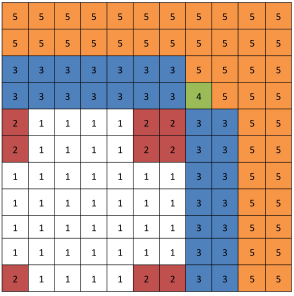
\includegraphics[width=0.5\linewidth]{../graphics/core}
\end{figure}
\end{frame}

\begin{frame}{Neutronics}
\begin{itemize}\vspace{-20pt}
\item Diffusion Approximation
\item Multigroup, $G=2$
\item Neglect Upscatter
\item $\chi(g=1)=1$
\item Solved using JFNK (GMRES) in \texttt{trilinos}
\end{itemize}\vspace{10pt}
Uncertainties:
\begin{itemize}
\item Aleatoric in interaction probability
\item Epistemic in measurements of $\sigma$
\end{itemize}
\end{frame}

\begin{frame}{Neutron Transport}{Two-Group, Two-Dimension, Diffusion Approximation}
\vspace{-30pt}
\begin{equation} \scriptsize
-\grad\cdot\qty( D_1(\bar x)\grad\phi_1(\bar x))+\qty(\xs{a}{1}(\bar x)+\xs{s}{1\to2}(\bar x))\phi_1(\bar x) = \frac{1}{k(\phi)}\sum_{g'=1}^2\nu_{g'}\xs{f}{g'}(\bar x)\phi_{g'}(\bar x) \nonumber
\end{equation}
\begin{equation}
-\grad \cdot\qty(D_2(\bar x)\grad \phi_2(\bar x))+\xs{a}{2}(\bar x)\phi_2(\bar x) = \xs{s}{1\to 2}(\bar x)\phi_1(\bar x)\nonumber
\end{equation}
\vspace{20pt}
\begin{equation}
-D\eval{\pdv{\phi^{\text{in}}}{x_i}}_{\partial D}=0,\hspace{5pt}i=1,2,\hspace{5pt}
    x\in\partial_\text{top}D\cup\partial_\text{right}D\nonumber
\end{equation}
\begin{equation}
\eval{\pdv{\phi}{x_i}}_{\partial D}=0,\hspace{5pt}i=1,2,\hspace{5pt}
    x\in\partial_\text{left}D\cup\partial_\text{bottom}D\nonumber
\end{equation}
\end{frame}

%\begin{frame}{Neutron Transport}{Two-Group, Two-Dimension, Diffusion Approximation}
%Quantity of Interest: $k$
%\begin{equation}
%k(\phi)=\sum_{g=1}^2\iint\limits_D\nu\xs{f}{g}\phi(\bar x)~d\bar x \nonumber
%\end{equation}
%\begin{itemize}
%\item Critical
%\item Subcritical
%\item Supercritical
%\end{itemize}
%\end{frame}

\begin{frame}{Neutron Transport}{Benchmark}\vspace{-20pt}
$k=1.00007605445$
\scriptsize
\begin{table}[h]
\centering
\begin{tabular}{c c | c c c c}
Region & Group & $D_g$ & $\Sigma_{a,g}$ & $\nu\Sigma_{f,g}$ & $\Sigma_s^{1,2}$ \\ \hline
1 & 1 & 1.255 & 8.252e-3 & 4.602e-3 & 2.533e-2 \\
 & 2 & 2.11e-1 & 1.003e-1 & 1.091e-1 & \\ \hline
2 & 1 & 1.268 & 7.181e-3 & 4.609e-3 & 2.767e-2 \\
 & 2 & 1.902e-1 & 7.047e-2 & 8.675e-2 & \\ \hline
3 & 1 & 1.259 & 8.002e-3 & 4.663e-3 & 2.617e-2 \\
 & 2 & 2.091e-1 & 8.344e-2 & 1.021e-1 & \\ \hline
4 & 1 & 1.259 & 8.002e-3 & 4.663e-3 & 2.617e-2 \\
 & 2 & 2.091e-1 & 7.3324e-2 & 1.021e-1 & \\ \hline
5 & 1 & 1.257 & 6.034e-4 & 0 & 4.754e-2 \\
 & 2 & 1.592e-1 & 1.911e-2 & 0 & 
\end{tabular}
\end{table}\normalsize
Introduce 10\% Uncertainty
\end{frame}

\section{UQ Methodology}
\begin{frame}{Uncertainty Quantification}{UQ Methods}\vspace{-20pt}
\begin{itemize}
\item Analog Monte Carlo
\item Stochastic Collocation on Sparse Grids
\item Anisotropic Stochastic Collocation
\end{itemize}
Uncertainty space
\[k(D_g,\Sigma_c^g,\nu\Sigma_f^g,\Sigma_s^{1\to2},\ldots) \to u(Y)\equiv u(Y_1,Y_2,\ldots,Y_N),Y\in\Gamma\]%\vspace{10pt}
Compare moments, $P(Y)=\prod_{n=1}^N \rho(Y_n)$
\[\expv{u^r}\equiv\int_\Omega u(Y)^rP(Y)d\Omega\]
\end{frame}

\begin{frame}{Uncertainty Quantification}{Monte Carlo}
\[\expv{u^r}\approx\frac{1}{M}\sum_{m=1}^M u\left(Y^{(m)}\right)^r\]
%TODO pdf of k?
\end{frame}

\begin{frame}{Uncertainty Quantification}{Stochastic Collocation}\vspace{-20pt}
\small
\begin{equation*}\label{approx}
u(Y)\approx u_{h,\eta,\Lambda(L)}(Y)=\sum_{k=0}^\eta u(Y^{(k)})\mathcal{L}_k(Y)
\end{equation*}
\begin{equation*}
\mathcal{L}_k(Y)=\prod_{n=1}^N \mathcal{L}_{k_n}(Y_n)
\end{equation*}
\begin{equation*}
\mathcal{L}_{k_n}(Y_n)=\prod_{j=1}^i \frac{Y_n-Y_n^{(i)}}{Y_n^{(k_n)}-Y_n^{(i)}}
\end{equation*}
\begin{equation*}
\expv{u(Y)}\approx\expv{u_h(Y)}=\sum_{k=1}^\eta w_k ~u_h\qty(Y^{(k)})
\end{equation*}
\end{frame}

\begin{frame}{Uncertainty Quantification}{Stochastic Collocation: Index Set $\Lambda(L)$}\vspace{-20pt}
\begin{itemize}
\item Tensor Product:\scriptsize\[\Lambda_\text{TP}(L)=\Big\{\bar p=[p_1,...,p_N]: \max_{1\leq n\leq N}p_n\leq L \Big\},\eta=(L+1)^N\]\normalsize
\item Total Degree: \scriptsize\[\Lambda_\text{TD}(L)=\Big\{\bar p=[p_1,...,p_N]:\sum_{n=1}^N p_n \leq L \Big\},\eta={L+N\choose N}\]\normalsize
\item Hyperbolic Cross: \scriptsize\[\Lambda_\text{HC}(L)=\Big\{\bar p=[p_1,...,p_N]:\prod_{n=1}^N p_n+1 \leq L+1 \Big\},\eta\leq (L+1)(1+\log(L+1))^{N-1}\]
\end{itemize}
\end{frame}

\begin{frame}{Uncertainty Quantification}{Stochastic Collocation: Index Set $\Lambda(L)$}\vspace{-20pt}
\begin{figure}[H]
\centering
  \begin{subfigure}[b]{0.32 \textwidth}
   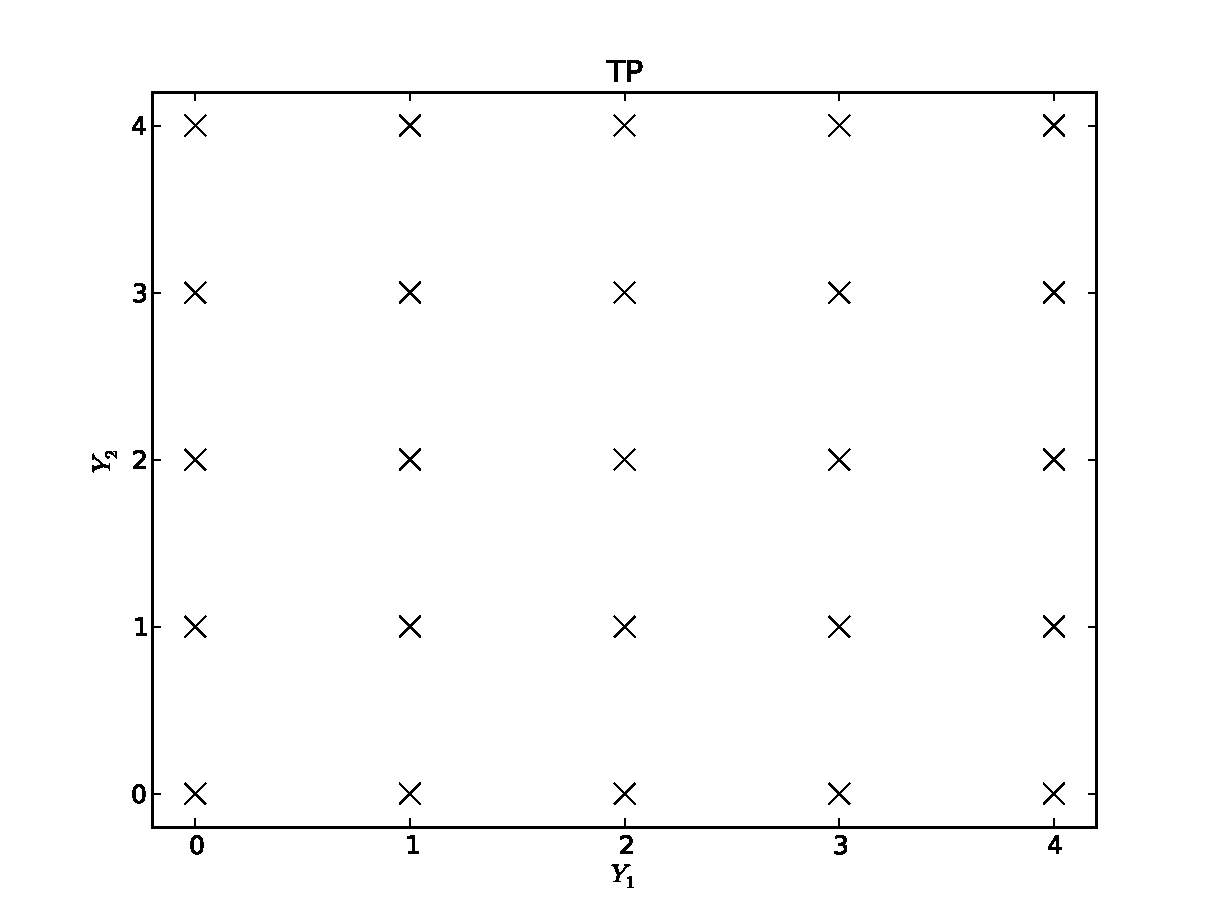
\includegraphics[width=\textwidth]{../graphics/TP}
   \caption{Tensor Product}
   \label{TP}
  \end{subfigure}
  \begin{subfigure}[b]{0.32 \textwidth}
   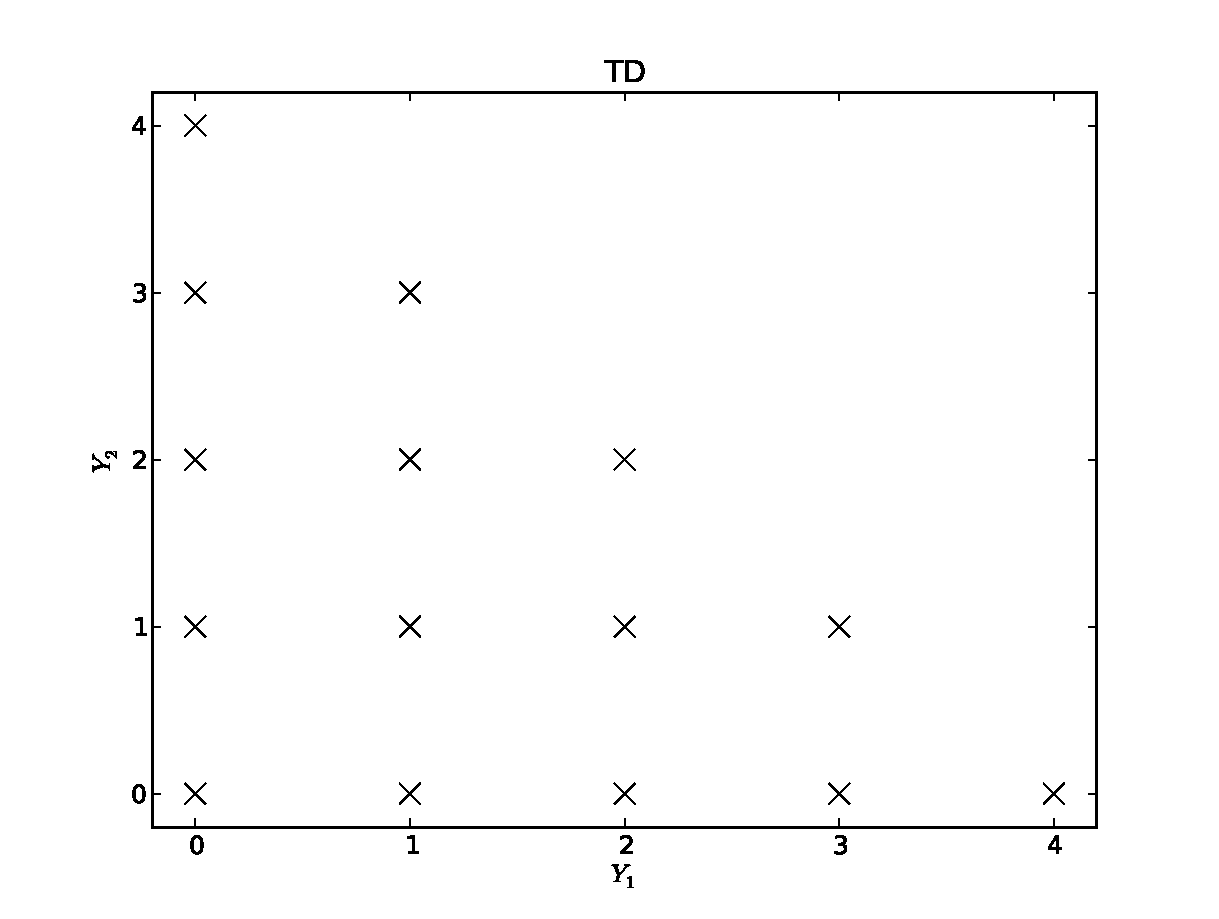
\includegraphics[width=\textwidth]{../graphics/TD}
   \caption{Total Degree}
   \label{TD}
  \end{subfigure}
  \begin{subfigure}[b]{0.32 \textwidth}
   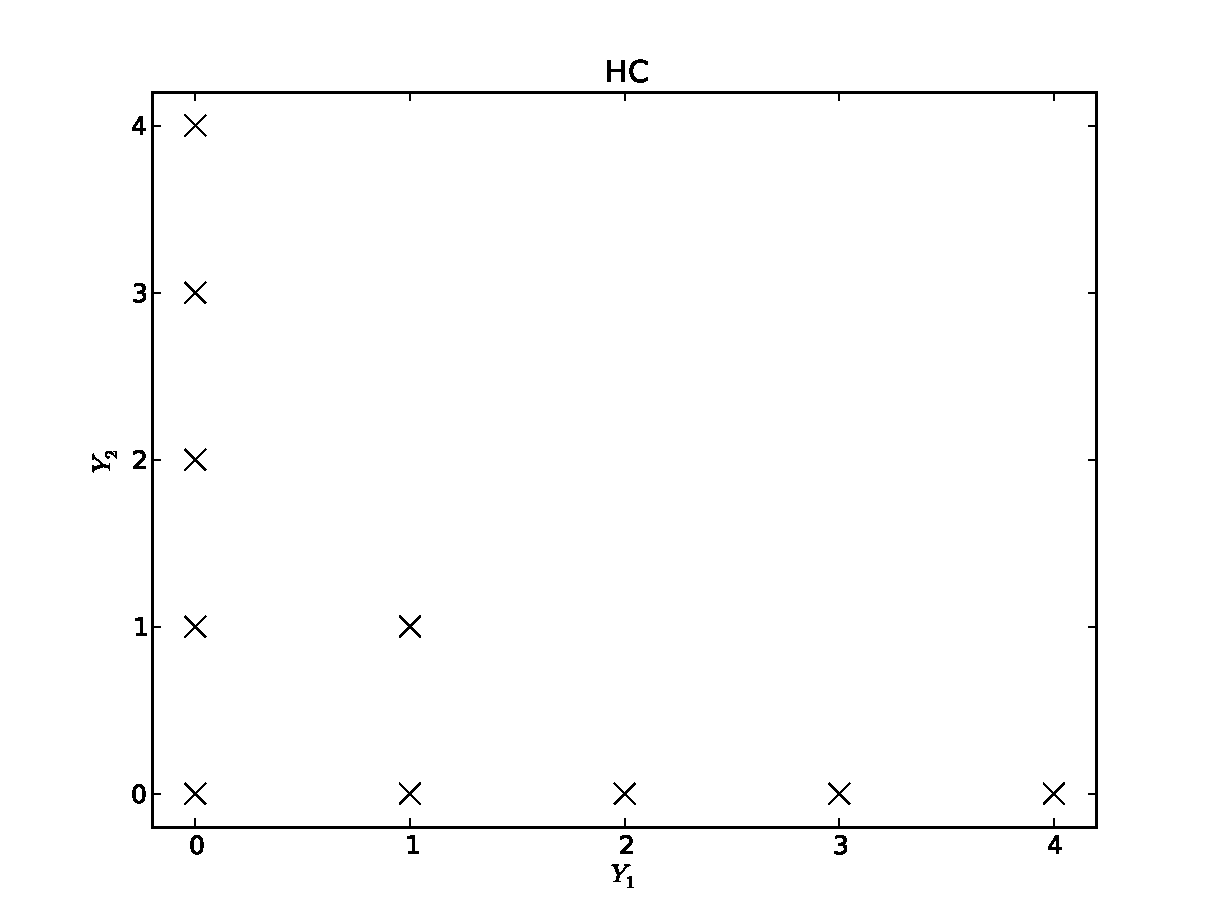
\includegraphics[width=\textwidth]{../graphics/HC}
   \caption{Hyperbolic Cross}
   \label{HC}
  \end{subfigure}
  \caption{Index Set Examples: $N=2,L=4$}
  \label{indexsets}
\end{figure}
\end{frame}

\begin{frame}{Uncertainty Quantification}{Stochastic Collocation on Sparse Grids}\normalsize\vspace{-20pt}
\begin{equation*}
u(Y)\approx\mathcal{S}_{N,\Lambda(L)}[u](Y)=\sum_{\boldsymbol{i}\in\Lambda(L)}c(\boldsymbol{i})\bigotimes_{n=1}^N\mathcal{U}_{n,p(i_n)}[u](Y),
\end{equation*}
\begin{equation*}
c(\boldsymbol{i})=\sum_{\substack{\boldsymbol{j}=\{0,1\}^N,\\ \boldsymbol{i}+\boldsymbol{j}\in\Lambda(L)}}(-1)^{|\boldsymbol{j}|_1},
\end{equation*}
\begin{align*}
\bigotimes_{n=1}^N\mathcal{U}_{n,p(i_n)}[u](Y)&\equiv\sum_{k_1=0}^{p(i_1)}\cdots\sum_{k_N=0}^{p(i_N)}u_h\qty(Y^{(k_1)},\cdots,Y^{(k_N)})\prod_{n=1}^N \mathcal{L}_{k_n}(Y_n),\\
  &=\sum_{k}^{p(\vec i)}u_h\qty(Y^{(k)})\mathcal{L}_k(Y),
\end{align*}
\end{frame}

\begin{frame}{Uncertainty Quantification}{Stochastic Collocation on Sparse Grids}\normalsize\vspace{-20pt}
\begin{figure}[H]
\centering
  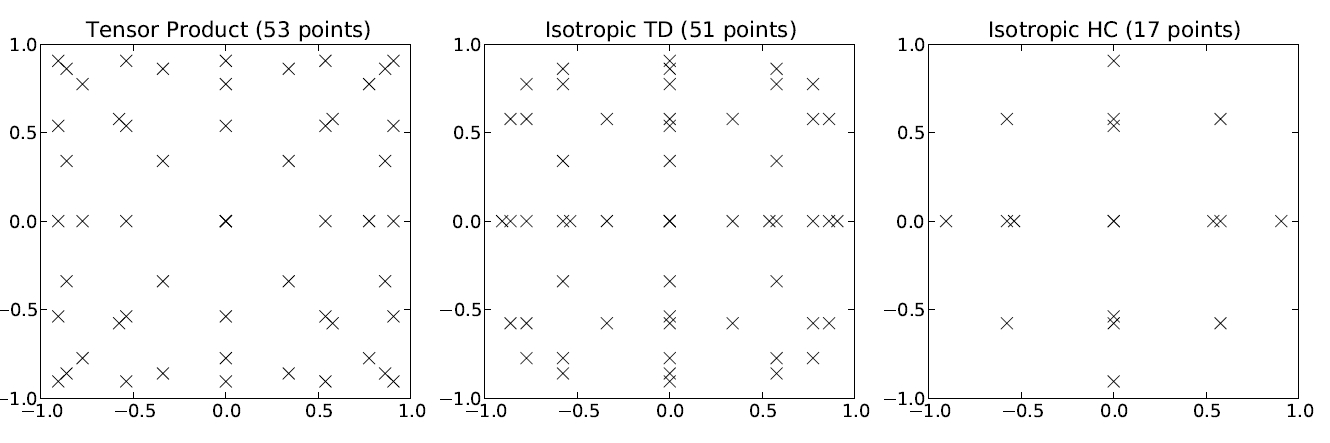
\includegraphics[width=\linewidth]{../graphics/jpgsparse}
  \caption{Sparse Grids, $N=2,L=4,p(i)=i$, Legendre points}
  \label{collsets}
\end{figure}
\end{frame}

\begin{frame}{Uncertainty Quantification}{Stochastic Collocation on Sparse Grids}\normalsize\vspace{-20pt}
\begin{table}
\centering
\begin{tabular}{c|c|c|c c|c c}
 &  & TP & \multicolumn{2}{|c|}{TD} & \multicolumn{2}{|c}{HC} \\ 
$N$ & $L$ & $\qty|\Lambda(L)|$ & $\qty|\Lambda(L)|$ & $\eta$ & $\qty|\Lambda(L)|$ & $\eta$\\ \hline
3 & 4 & 125    & 35    & 165   & 16 & 31\\
 & 8   & 729    & 165  & 2,097  & 44 & 153\\
 & 16 & 4,913  & 969   & 41,857 & 113 & 513\\
 & 32 & 35,737 & 6,545 & 1,089,713 & 309 & 2,181\\ \hline
5 & 2 & 293 & 21 & 61 & 11 & 11\\
 & 4 & 3,125 & 126 & 781 & 31 & 71\\
 & 8 & 59,049 & 1,287 & 28,553 & 111 & 481 
\end{tabular}
\caption{Index Set and Collocation Size Comparison}
\label{compIS}
\end{table}
\end{frame}

\begin{frame}{Uncertainty Quantification}{Anisotropic Sparse Grids}\normalsize\vspace{-20pt}
%\begin{equation}
%\qty|\vec\alpha|_1\equiv\frac{1}{N}\sum_{n=1}^N \alpha_n,
%\end{equation}
\begin{equation*}
\tilde\Lambda_\text{TD}(L)=\Big\{\bar p=[p_1,...,p_N]:\sum_{n=1}^N \alpha_n p_n \leq \qty|\vec\alpha|_1 L \Big\}
\end{equation*}
\begin{equation*}
\tilde\Lambda_\text{HC}(L)=\Big\{\bar p=[p_1,...,p_N]:\prod_{n=1}^N \qty(p_n+1)^{\alpha_n} \leq \qty(L+1)^{\qty|\vec\alpha|_1} \Big\}
\end{equation*}
\end{frame}

\section{Results}
\begin{frame}{Sample Results}{Attenuation,  $u(Y)=\prod_n^N \exp(-Y_n)$ ($N=5$)}
  \begin{figure}[h!]
    \centering
    \begin{subfigure}[b]{0.49 \textwidth}
      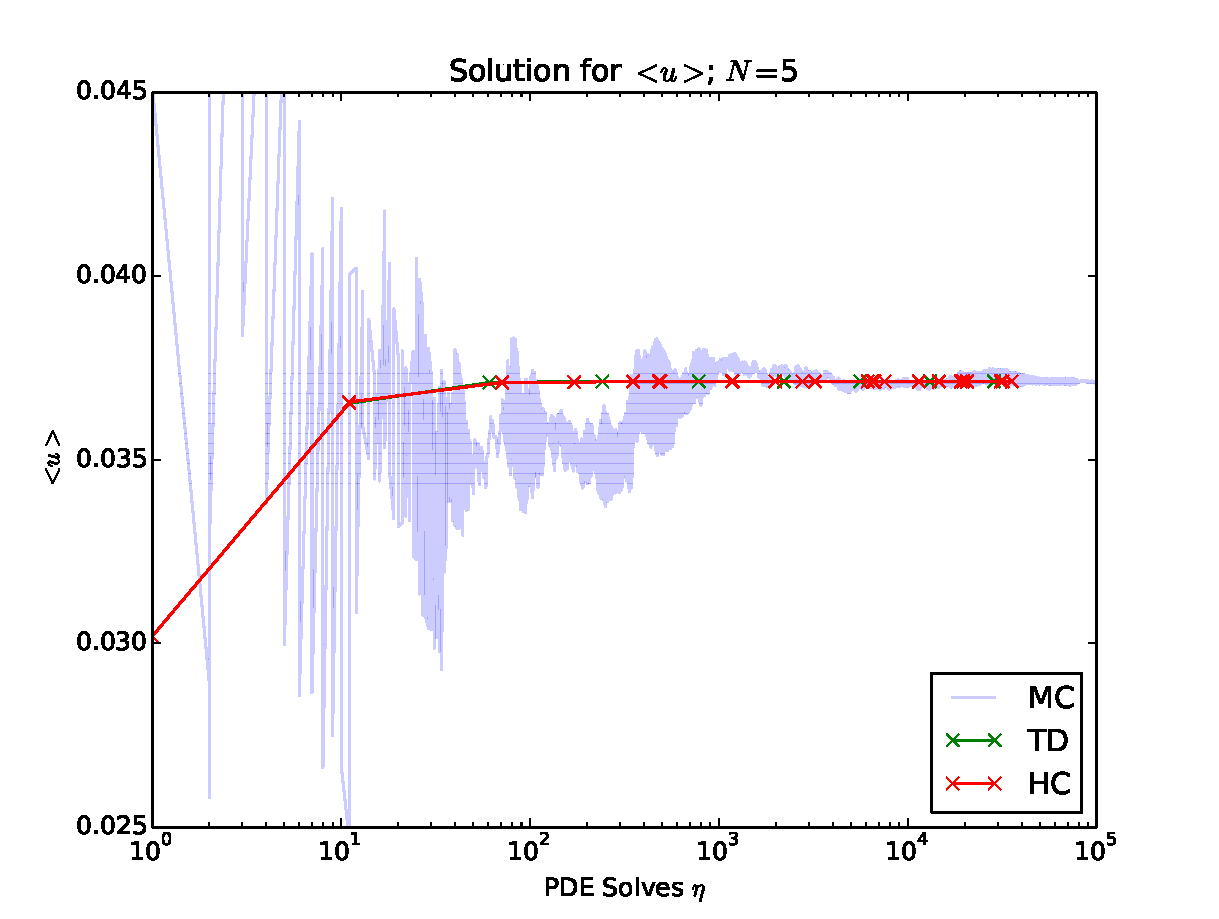
\includegraphics[width=\textwidth]{../graphics/attenuate_N5_soln}
      \caption{$<u>$ Values}
      \label{err_5}
    \end{subfigure}
    \begin{subfigure}[b]{0.49 \textwidth}
      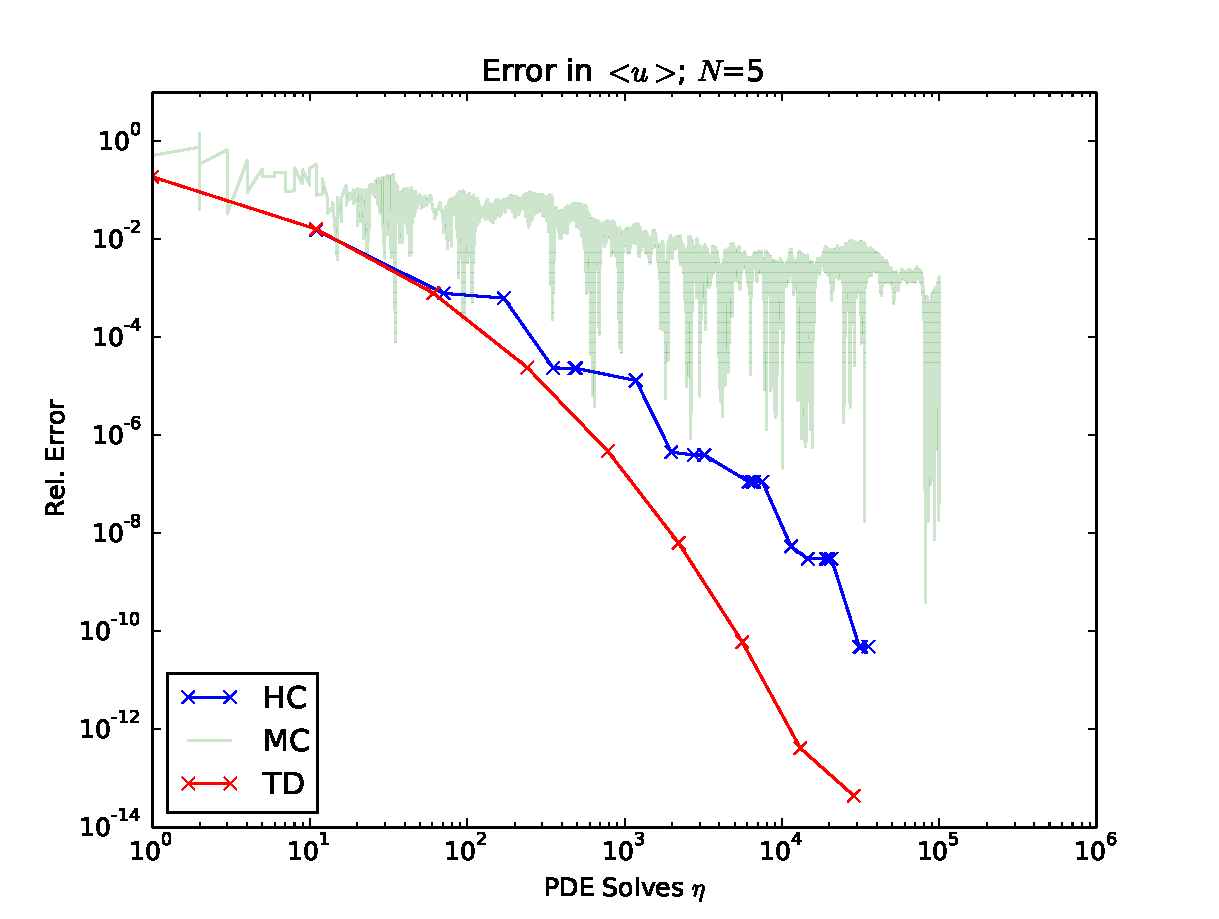
\includegraphics[width=\textwidth]{../graphics/attenuate_N5_conv}
      \caption{Error in $<u>$}
      \label{err_14}
    \end{subfigure}
  \end{figure}
\end{frame}

\begin{frame}{Results}{$<k>$ Values}
  \begin{figure}[h!]
    \centering
    \begin{subfigure}[b]{0.49 \textwidth}
      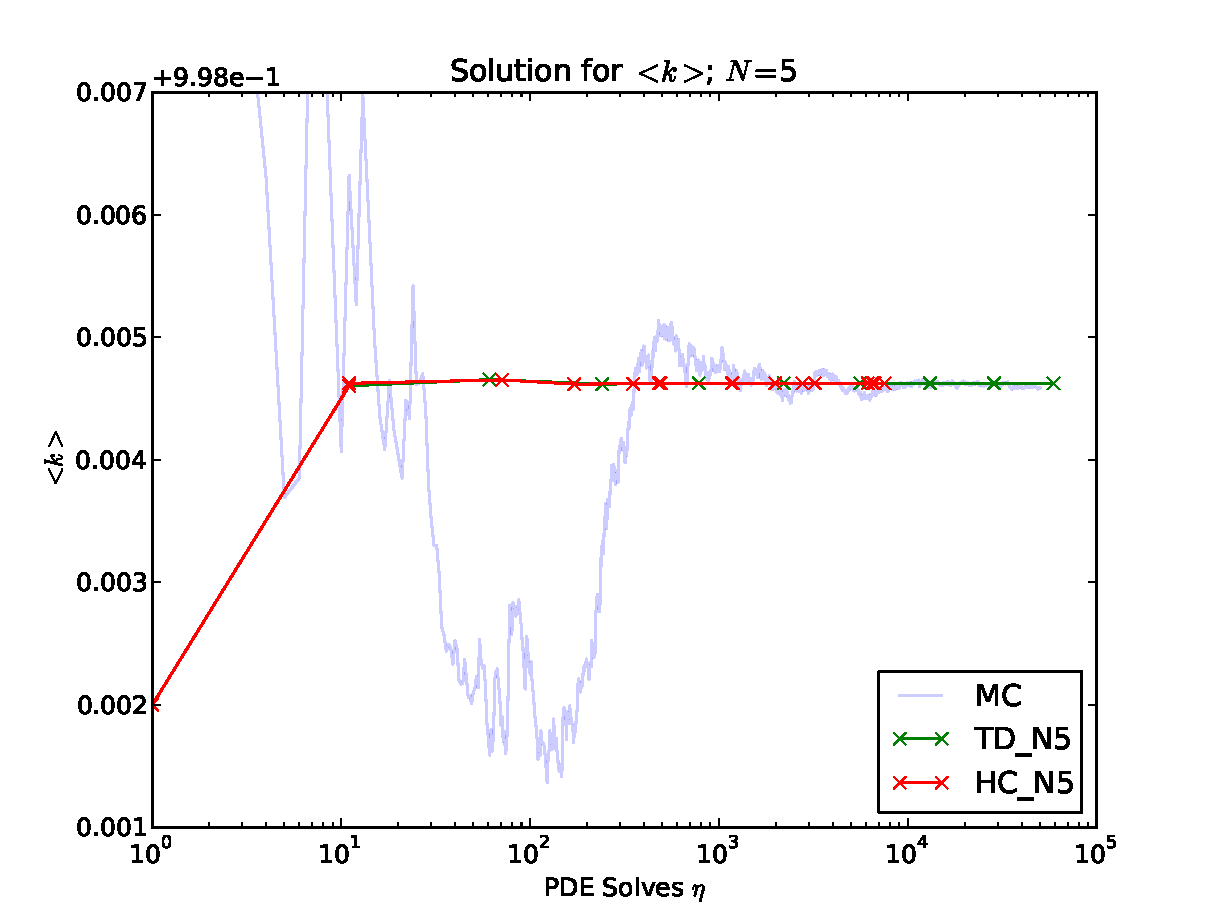
\includegraphics[width=\textwidth]{../graphics/soln_5}
      \caption{$<k>$, N=5}
      \label{soln_5}
    \end{subfigure}
    \begin{subfigure}[b]{0.49 \textwidth}
      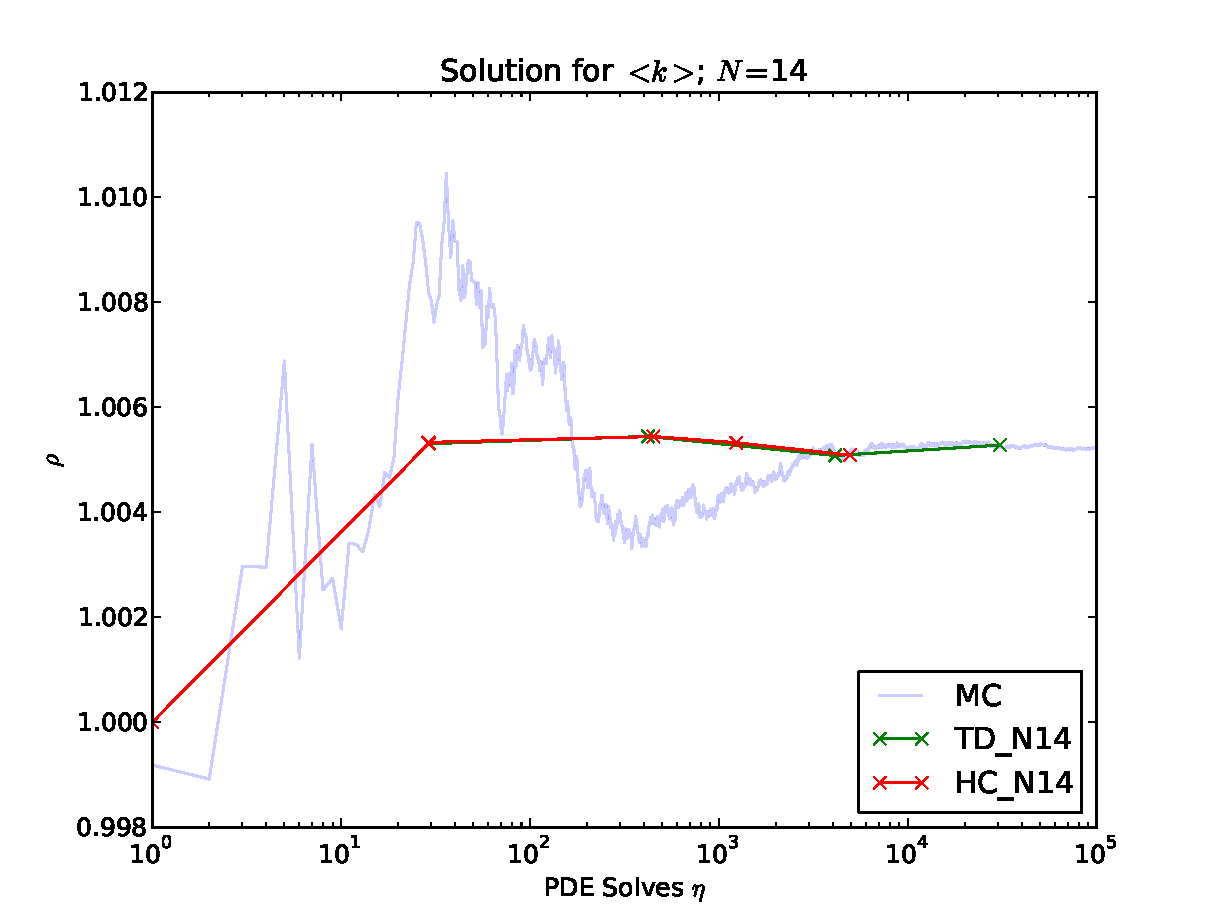
\includegraphics[width=\textwidth]{../graphics/soln_14}
      \caption{$<k>$, N=14}
      \label{soln_14}
    \end{subfigure}
  \end{figure}
\end{frame}

\begin{frame}{Results}{$<k>$ Convergence}
  \begin{figure}[h!]
    \centering
    \begin{subfigure}[b]{0.49 \textwidth}
      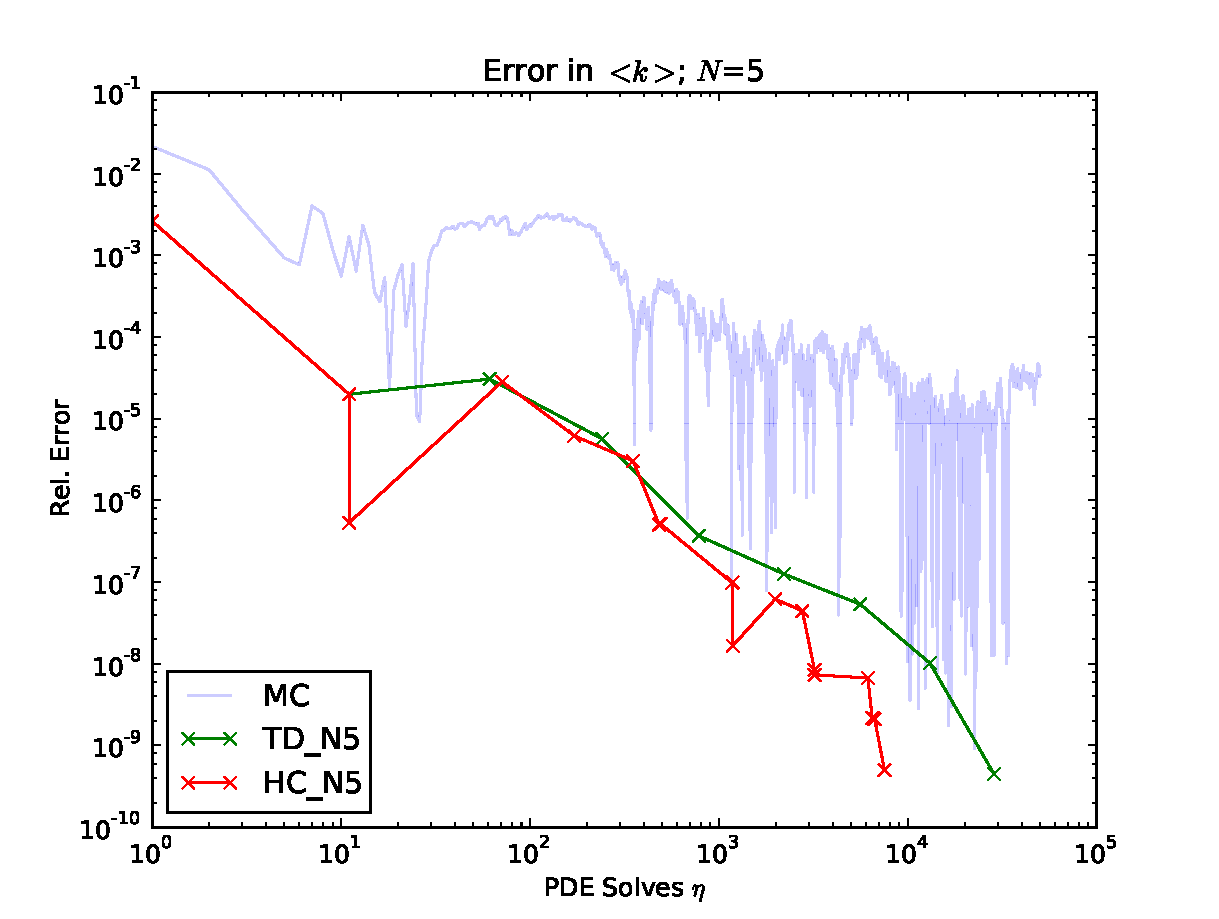
\includegraphics[width=\textwidth]{../graphics/err_5}
      \caption{Error in $<k>$, N=5}
      \label{err_5}
    \end{subfigure}
    \begin{subfigure}[b]{0.49 \textwidth}
      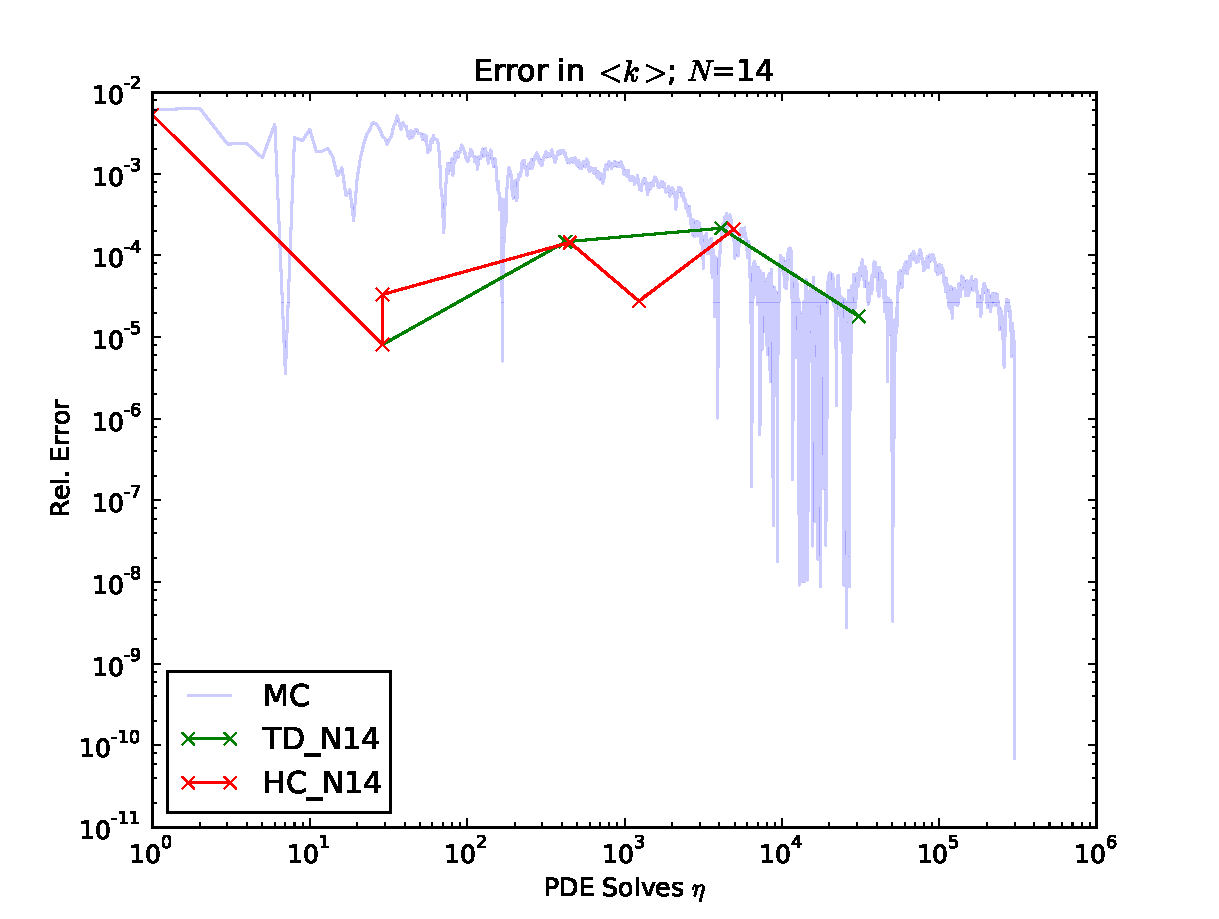
\includegraphics[width=\textwidth]{../graphics/err_14}
      \caption{Error in $<k>$, N=14}
      \label{err_14}
    \end{subfigure}
  \end{figure}
\end{frame}

\begin{frame}{Results}{var$(k)$ Values}
  \begin{figure}[h!]
    \centering
    \begin{subfigure}[b]{0.49 \textwidth}
      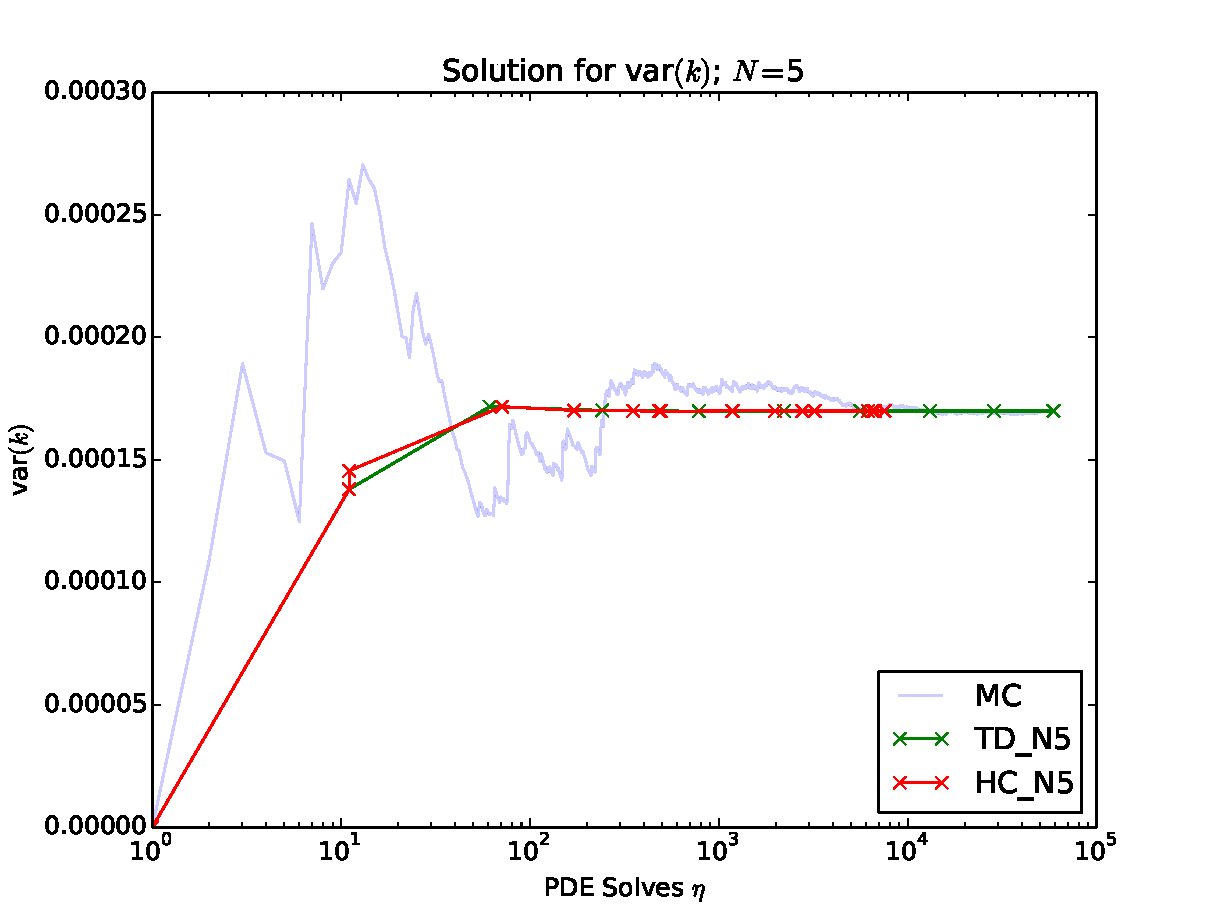
\includegraphics[width=\textwidth]{../graphics/N5_iso_var_vals}
      \caption{var$(k)$, N=5}
      \label{vsoln_5}
    \end{subfigure}
    \begin{subfigure}[b]{0.49 \textwidth}
      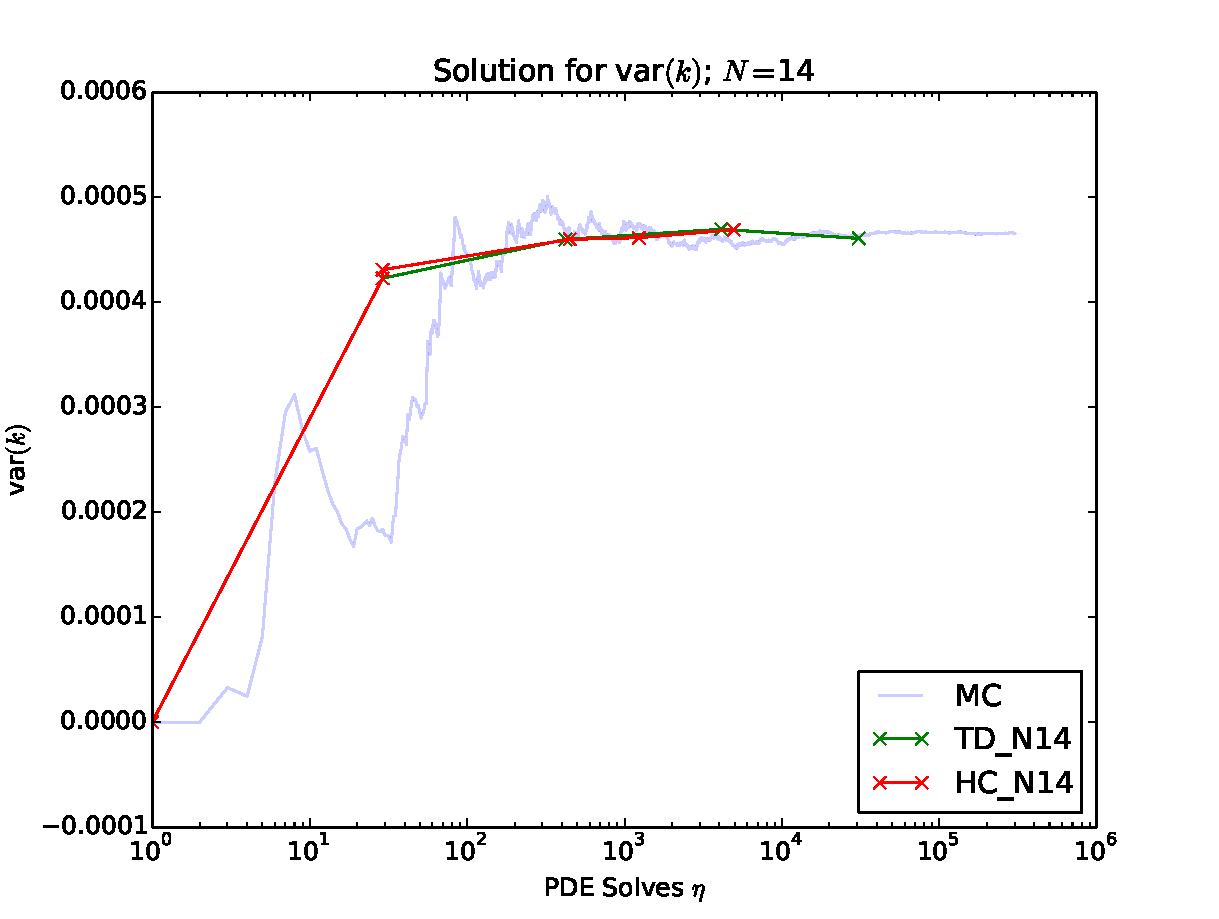
\includegraphics[width=\textwidth]{../graphics/N14_iso_var_vals}
      \caption{var$(k)$, N=14}
      \label{vsoln_14}
    \end{subfigure}
  \end{figure}
\end{frame}

\begin{frame}{Results}{var$(k)$ Convergence}
  \begin{figure}[h!]
    \centering
    \begin{subfigure}[b]{0.49 \textwidth}
      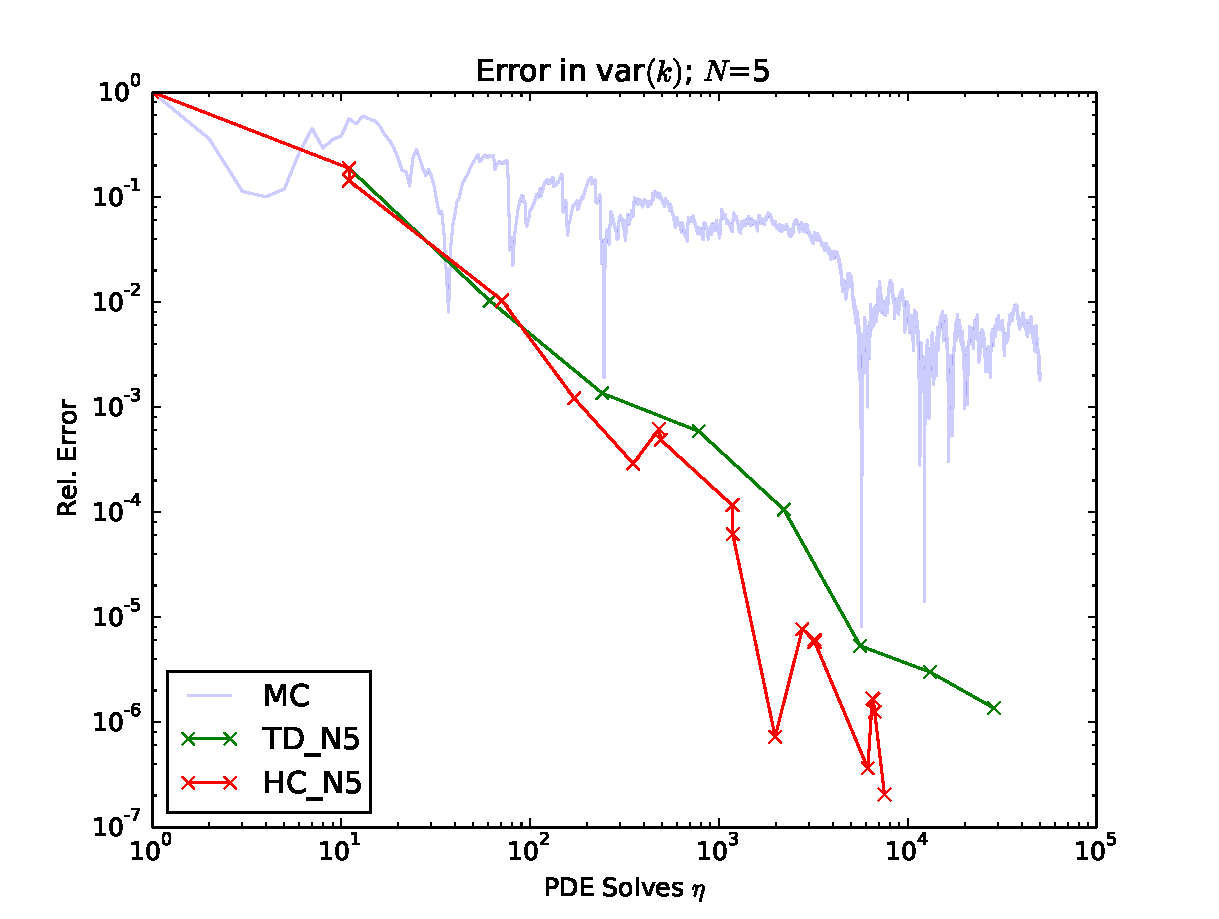
\includegraphics[width=\textwidth]{../graphics/N5_iso_var_errs}
      \caption{Error in var$(k)$, N=5}
      \label{verr_5}
    \end{subfigure}
    \begin{subfigure}[b]{0.49 \textwidth}
      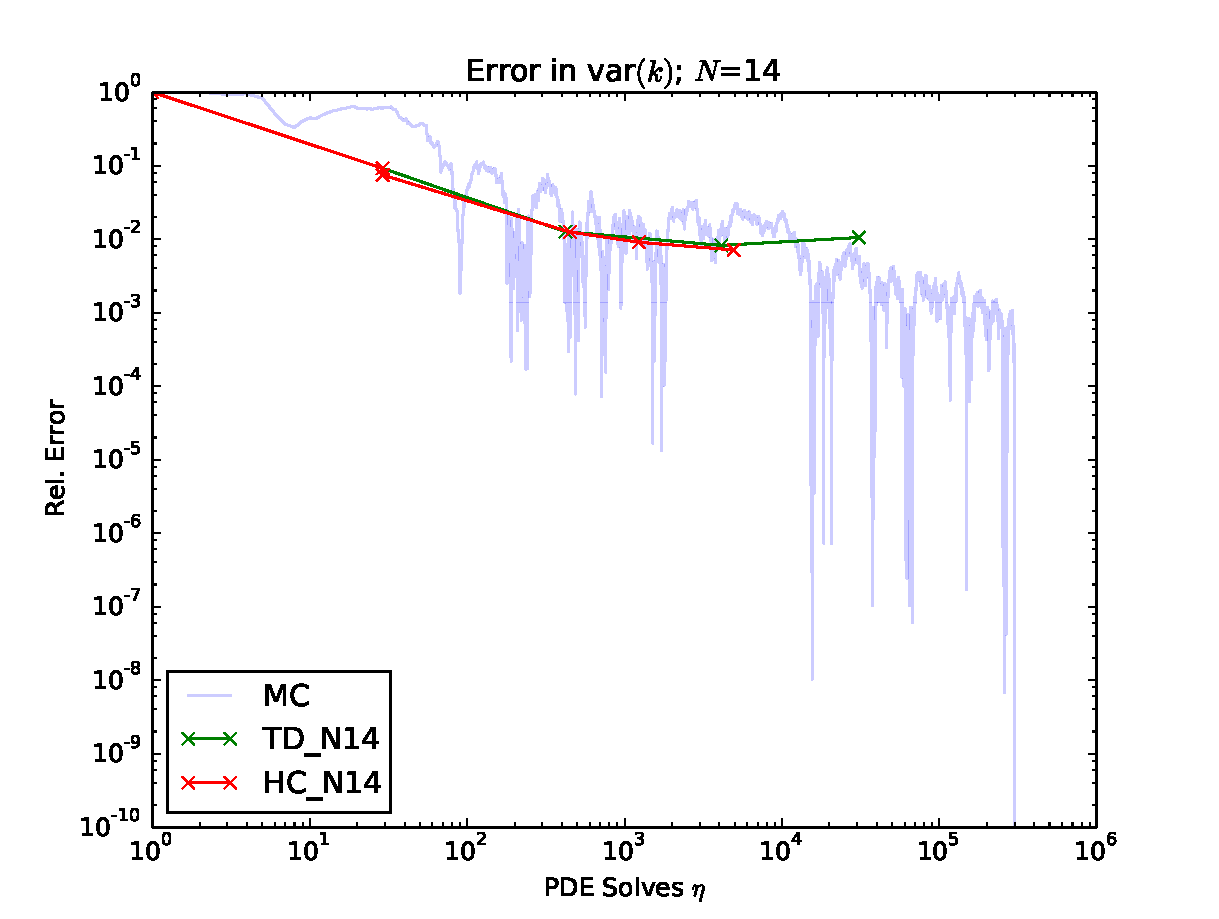
\includegraphics[width=\textwidth]{../graphics/N14_iso_var_errs}
      \caption{Error in var$(k)$, N=14}
      \label{verr_14}
    \end{subfigure}
  \end{figure}
\end{frame}

\section{Ongoing Work}
\begin{frame}{Continuing Efforts}\vspace{-50pt}
\begin{itemize}
\item Increased Material Complexity
\item Adaptive  Anisotropic Grids
\item HDMR
\item Multiphysics (Neutronics, Thermal Hydraulics, Materials)
\end{itemize}
\end{frame}

\section{}
\begin{frame}{}

\end{frame}

\begin{frame}{Sample Results}{Attenuation,  $u(Y)=\prod_n^N \exp(-Y_n)$ ($N=5$)}
  \begin{figure}[h!]
    \centering
    \begin{subfigure}[b]{0.49 \textwidth}
      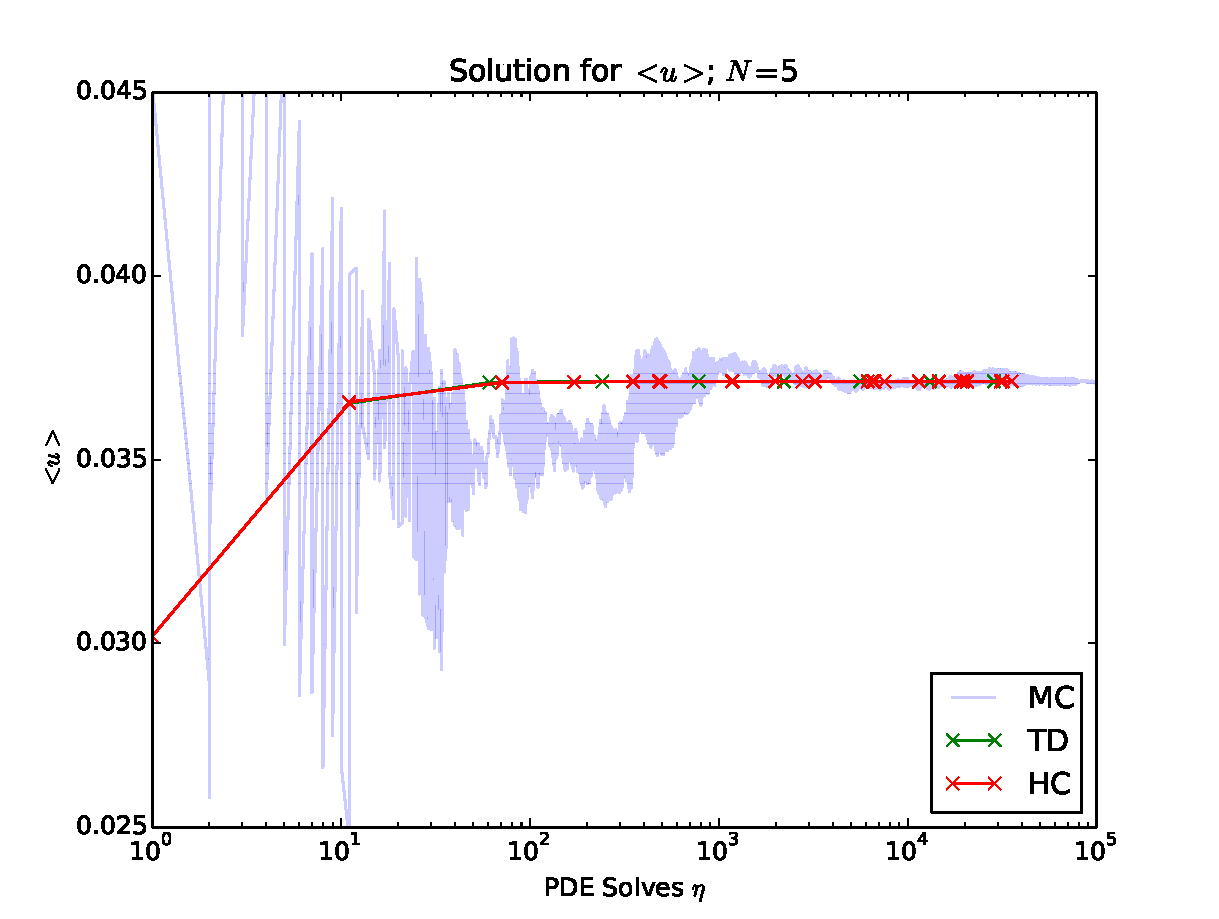
\includegraphics[width=\textwidth]{../graphics/attenuate_N5_soln}
      \caption{$<u>$ Values}
      \label{err_5}
    \end{subfigure}
    \begin{subfigure}[b]{0.49 \textwidth}
      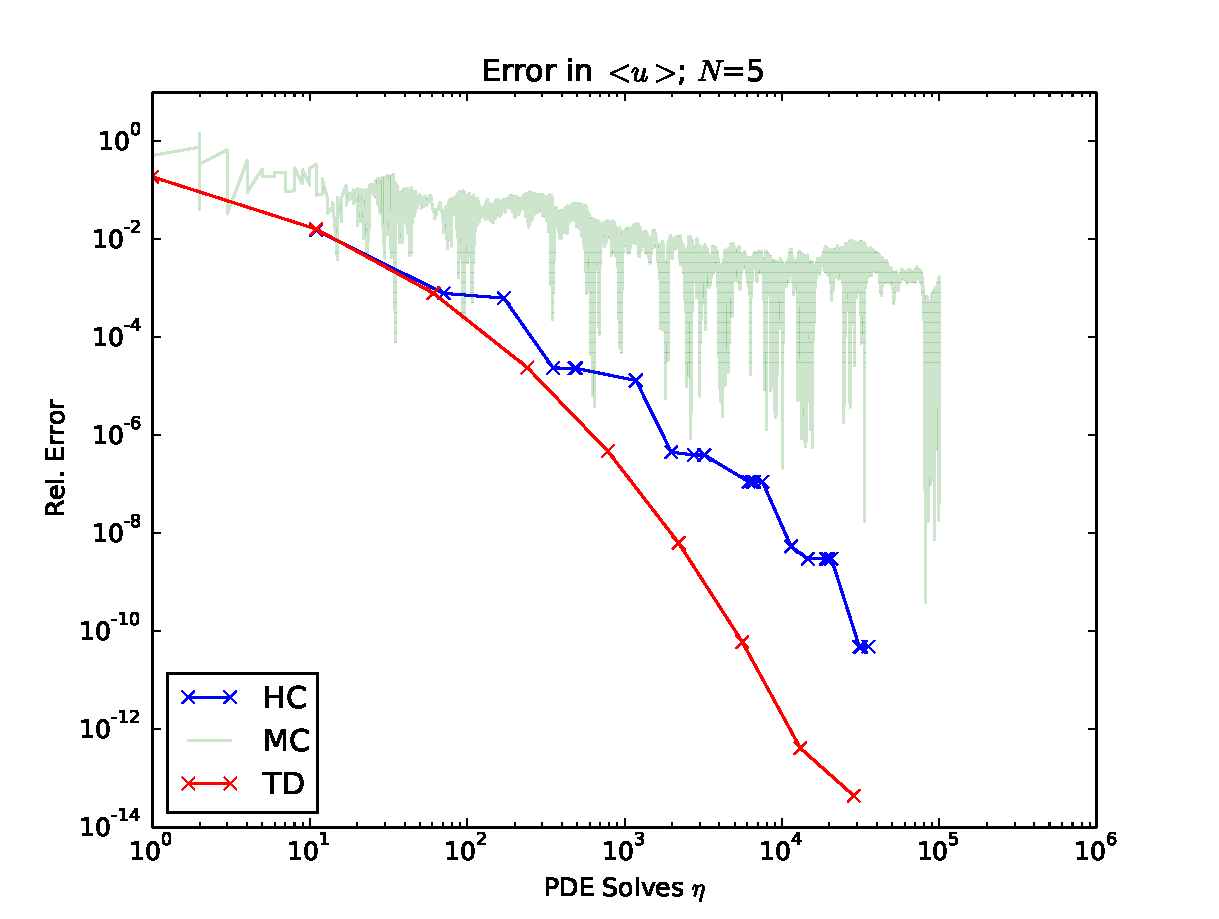
\includegraphics[width=\textwidth]{../graphics/attenuate_N5_conv}
      \caption{Error in $<u>$}
      \label{err_14}
    \end{subfigure}
  \end{figure}
\end{frame}
%
%\begin{frame}{Additional Results}{Projectile with Drag ($N=8$)}
%  \begin{figure}[h!]
%    \centering
%    \begin{subfigure}[b]{0.49 \textwidth}
%      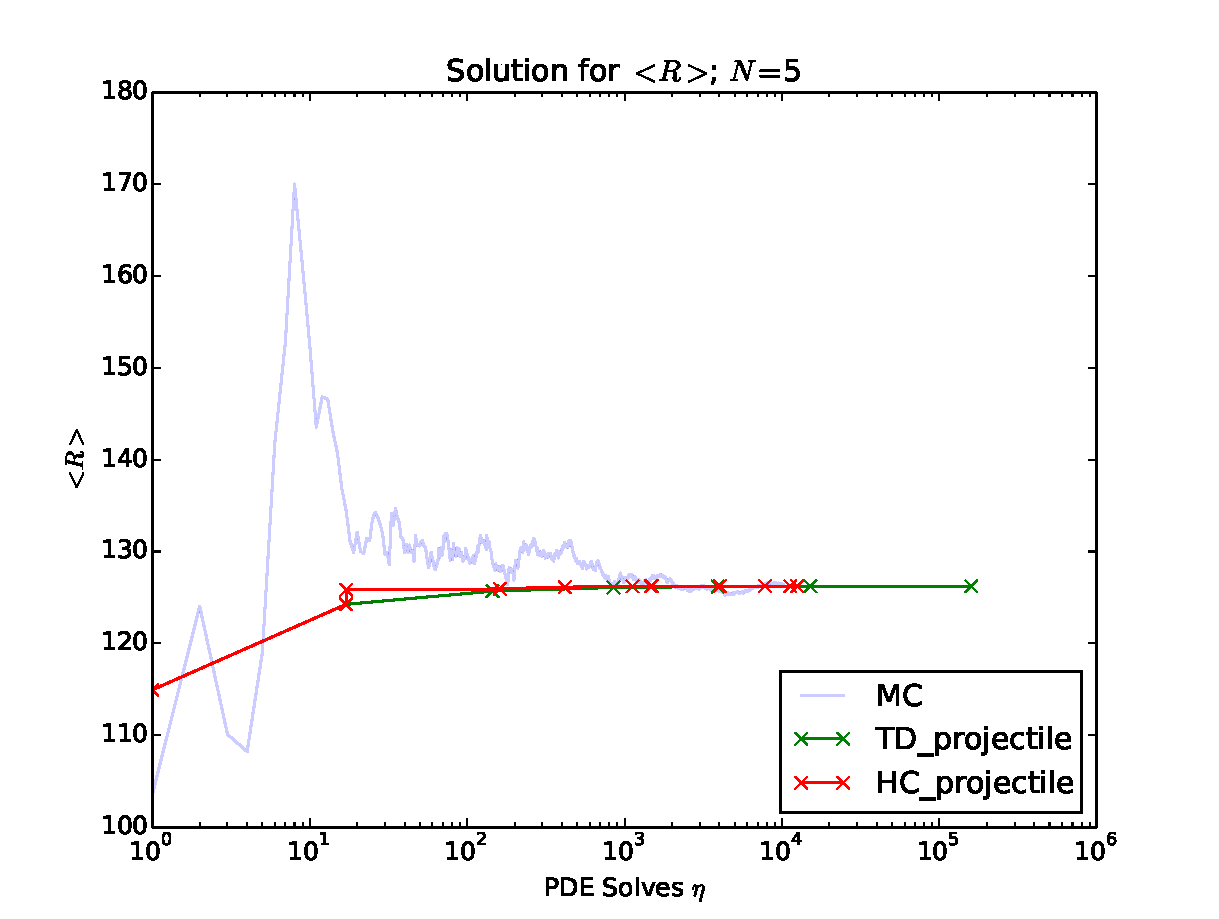
\includegraphics[width=\textwidth]{../graphics/projectile_solns}
%      \caption{$<R>$ Values}
%      \label{err_5}
%    \end{subfigure}
%    \begin{subfigure}[b]{0.49 \textwidth}
%      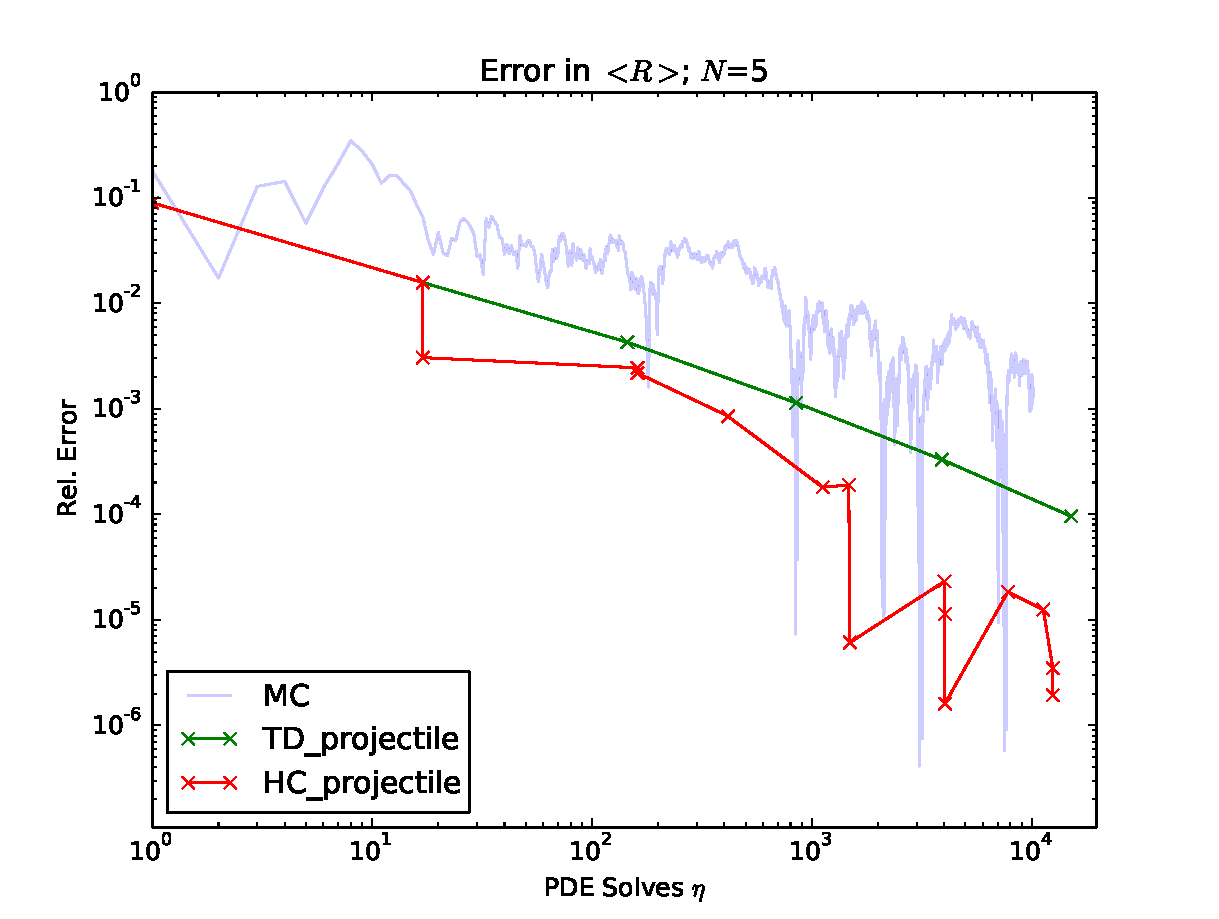
\includegraphics[width=\textwidth]{../graphics/projectile_errs}
%      \caption{Error in $<R>$}
%      \label{err_14}
%    \end{subfigure}
%  \end{figure}
%\end{frame}

\end{document}


